\documentclass[fontsize=12pt,toc=bibliography, notitlepage]{scrreprt}

\usepackage[english]{babel}
\usepackage{ucs}
\usepackage[utf8x]{inputenc}
\usepackage[bookmarksopen=true,
			bookmarks=true,
			plainpages=false,
        	pdfpagelabels=true,
			colorlinks=true,
			linkcolor=black,
			citecolor=black,
        	filecolor=black,
        	urlcolor=blue]{hyperref}
\usepackage{graphicx}
\usepackage{float}
\usepackage{listings}
\usepackage{color}
\usepackage{tikz}

\title{Knapsack Genetic Algorithm}
\subtitle{Artificial Intelligence 2}
\author{Fabian Meyer}
\date{\today \\ HTWG Konstanz}

\lstdefinestyle{MyJavaStyle}{
  belowcaptionskip=1\baselineskip,
  breaklines=true,
  frame=single,
  captionpos=b,
  numbers=left,
  xleftmargin=\parindent,
  language=Java,
  showstringspaces=false,
  basicstyle=\footnotesize\ttfamily,
  keywordstyle=\bfseries\color{green!40!black},
  commentstyle=\itshape\color{purple!40!black},
  identifierstyle=\color{blue},
  stringstyle=\color{orange}
}
\lstset{escapechar=@,style=MyJavaStyle}

\newcommand{\refnn}[1]{\ref{#1} \nameref{#1}}

\begin{document}

\maketitle
\begin{abstract}
The performance of a genetic search algorithm highly depends on its parameters, such as generation count, number of individuals, etc. In this paper the influence of these parameters on a algorithm solving a multidimensional knapsack problem is discussed.
\end{abstract}
\tableofcontents

\chapter{Genetic Algorithm}
\label{chap:genetic-algorithm}

\section{Implementation}
\label{sec:implementation}

The Genetic Algorithm (GA) is built upon various modules, which influence its behaviour. \\
The key features of the GA described in this paper are:
\begin{itemize}
	\item gene representation using boolean array
	\item pure random initial population
	\item roulette wheel selection of parents
	\item uniform crossover to generate children
	\item elitism to select individuals, which die
	\item mutation by probability for each child; only one single randomly chosen gene per child
	\item repairing individuals, which do not meet constraints
	\item fitness of individual = profit of individual
\end{itemize}

\section{Parameter}
\label{sec:parameter}
This implementation of the genetic algorithm (see \refnn{sec:implementation}) is customizable over various parameters. These include:
\begin{itemize}
	\item \nameref{subsec:mutation-probability}
	\item \nameref{subsec:breed-probability}
	\item \nameref{subsec:population-size}
	\item \nameref{subsec:algorithm-duration}
\end{itemize}
These parameters strongly influence the performance of the algorithm related to its speed and quality. In the following the parameters and their influence are discussed.\\
All diagrams show \textbf{problem 0} of the mknapcb1.txt from the OR library, but the results are applicable for all other problems. The x-axis shows the generation of the population and the y-axis shows the mean profit of the population.

\subsection{High quality configuration}
\label{subsec:good-config}
The following configuration generates good solutions for the given problem in reasonable time: \\ \\
\begin{tabular}{ |l|l| }
	\hline
	Breed probability & 0.8 \\ \hline
	Mutation probability & 0.0001 \\ \hline
	Generation count & 1000 \\ \hline
	Population size & 300 \\ \hline
\end{tabular}
\begin{figure}[H]
	\centering
	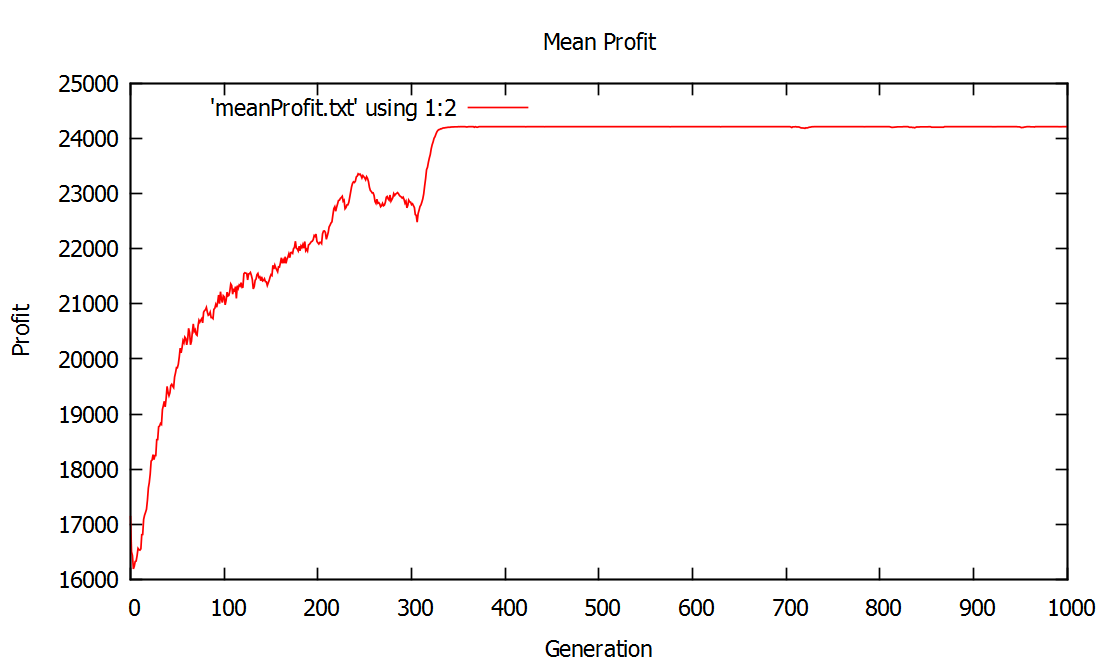
\includegraphics[width=400px]{images/good-config.png}
	\caption{High quality configuration}
	\label{fig:good-config}
\end{figure}
\textbf{Time taken: 13719ms}.\\
The generation count could be reduced to increase the speed of the algorithm, but like this its more obvious to see that the algorithm converges.

\subsection{Mutation Probability}
\label{subsec:mutation-probability}
Multiple tests showed that the mutation probability should be very low (e.g. 0.0001), else the algorithm never really converges against the optimal solution due to too much randomness.\\
\autoref{fig:mutation-high} shows the following configuration:\\ \\
\begin{tabular}{ |l|l| }
	\hline
	Breed probability & 0.8 \\ \hline
	Mutation probability & 0.2 \\ \hline
	Generation count & 1000 \\ \hline
	Population size & 300 \\ \hline
\end{tabular}
\begin{figure}[H]
	\centering
	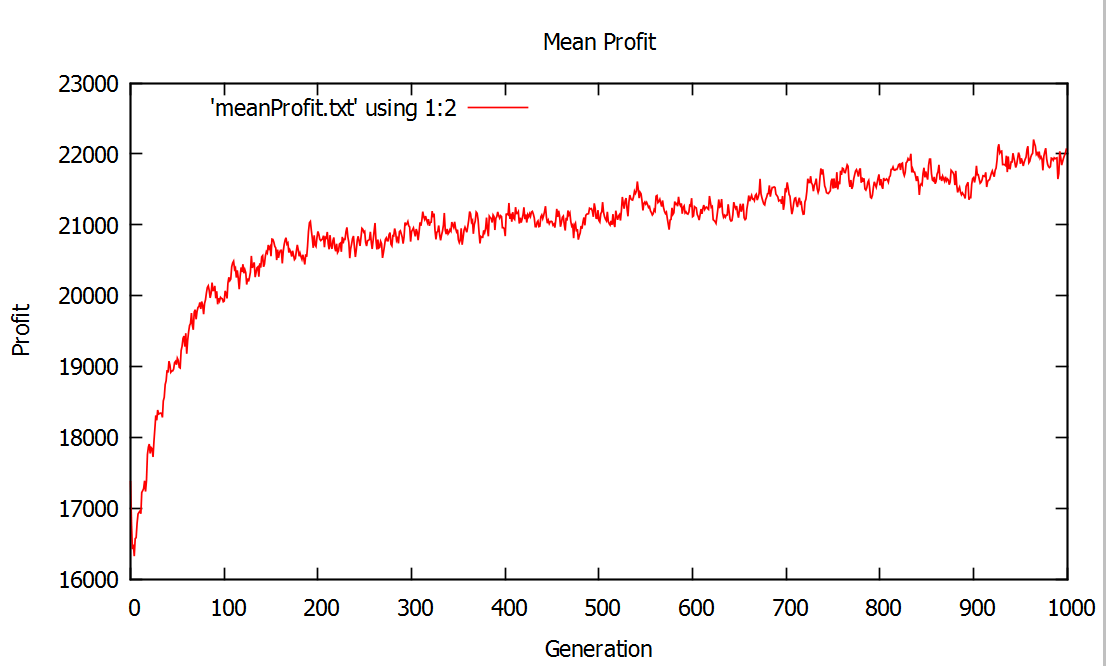
\includegraphics[width=400px]{images/mutation-high.png}
	\caption{High mutation probability}
	\label{fig:mutation-high}
\end{figure}
This figure shows that the algorithm does converge very slowly and there is much noise in the graph. This becomes especially clear if we look at \autoref{fig:good-config}.
The high quality configuration has the same parameters as shown in the table above, except that the mutation probability there is \textbf{0.0001}. The graph of \autoref{fig:good-config} has much less noise in it and converges much faster than the graph of \autoref{fig:mutation-high}. The low mutation approach also reaches a much higher profit value in the same amount of generations.

\subsection{Breed Probability}
\label{subsec:breed-probability}
The breed probability should always be a high value (e.g. 0.8), so the population changes a lot. If the probability is too low (e.g. 0.1), the population takes much more generations to improve its overall fitness than with a high probability. Is the probability set too high (e.g. 1.0) , too many individuals of the population are replaced. This leads to also removing the fittest individiuums in the generation and the optimal solution is never reached.\\
\autoref{fig:breed-low} shows the following configuration:\\ \\
\begin{tabular}{ |l|l| }
	\hline
	Breed probability & 0.1 \\ \hline
	Mutation probability & 0.0001 \\ \hline
	Generation count & 1000 \\ \hline
	Population size & 300 \\ \hline
\end{tabular}
\begin{figure}[H]
	\centering
	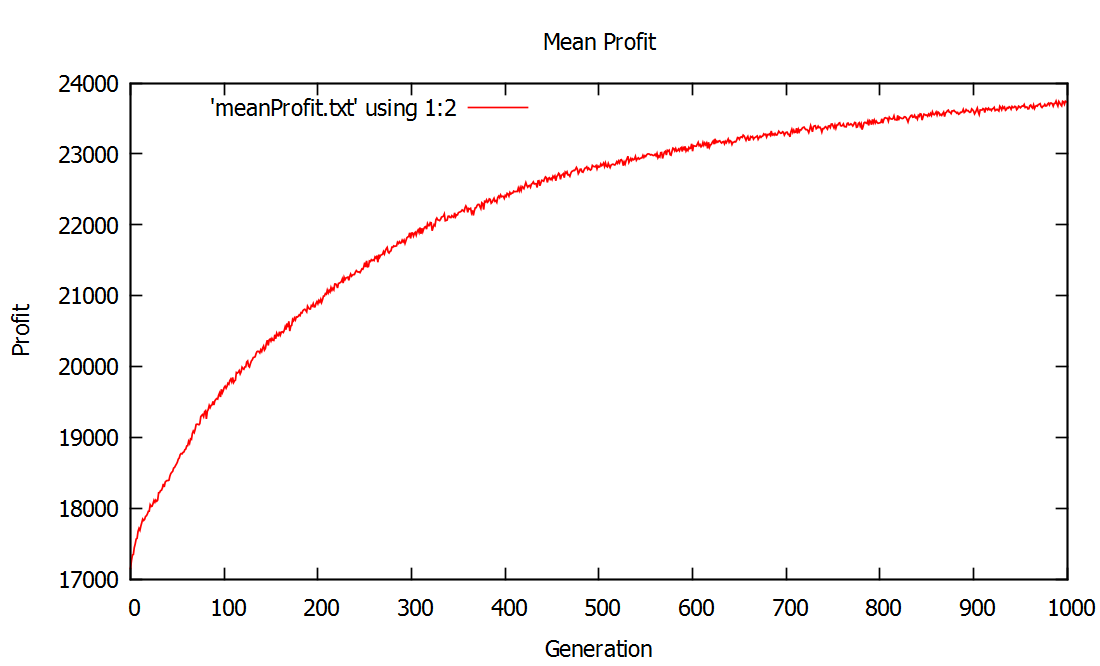
\includegraphics[width=400px]{images/breed-low.png}
	\caption{Low breed probability}
	\label{fig:breed-low}
\end{figure}
The graph of this figure converges very slowly and takes much processing until it reaches the optimum. In comparison to the high quality configuration shown in \autoref{fig:good-config}, which uses the same parameters as in the table above, but a higher
breed probability of 0.8, the graph of \autoref{fig:breed-low} converges much slower against the optimal solution.\\
\autoref{fig:breed-high} shows the experiment with too high breed probability (1.0).
\begin{figure}[H]
	\centering
	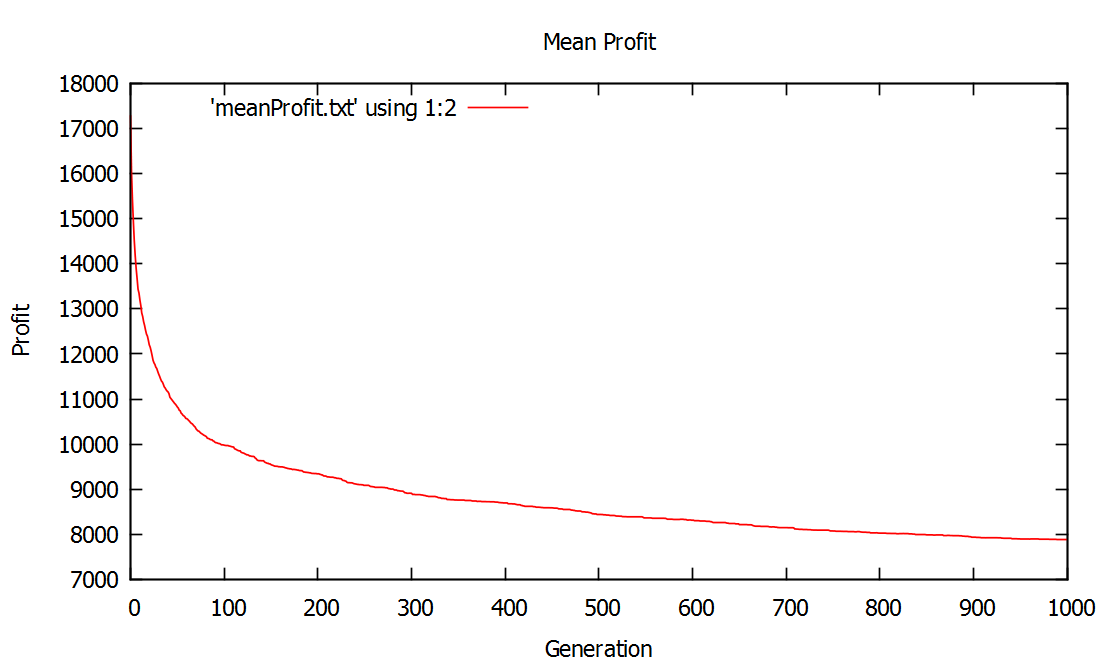
\includegraphics[width=400px]{images/breed-high.png}
	\caption{High breed probability}
	\label{fig:breed-high}
\end{figure}
The overall fitness in the population gets even worse. This is because a breed probability of 1.0 causes all individuals of the population being replaced - even the best. The resulting children may be better or worse than their parents, but after the mutation step it is highly probable that their fitness gets worse. The idea of breeding and mutation is to prevent being stuck at a local optimum. But if the algorithm also removes the best individuals, the overall fitness decreases.

\subsection{Population Size}
\label{subsec:population-size}
With a high population size there is plenty of gene diversity in the population, but the algorithm takes longer to calculate. A low population size leads to less diversity. If it is too low, the algorithm gets stuck in a local optimum, because some genes are missing in the population.\\
\autoref{fig:population-high} shows the following configuration: \\ \\
\begin{tabular}{ |l|l| }
	\hline
	Breed probability & 0.8 \\ \hline
	Mutation probability & 0.0001 \\ \hline
	Generation count & 1000 \\ \hline
	Population size & 1000 \\ \hline
\end{tabular}
\begin{figure}[H]
	\centering
	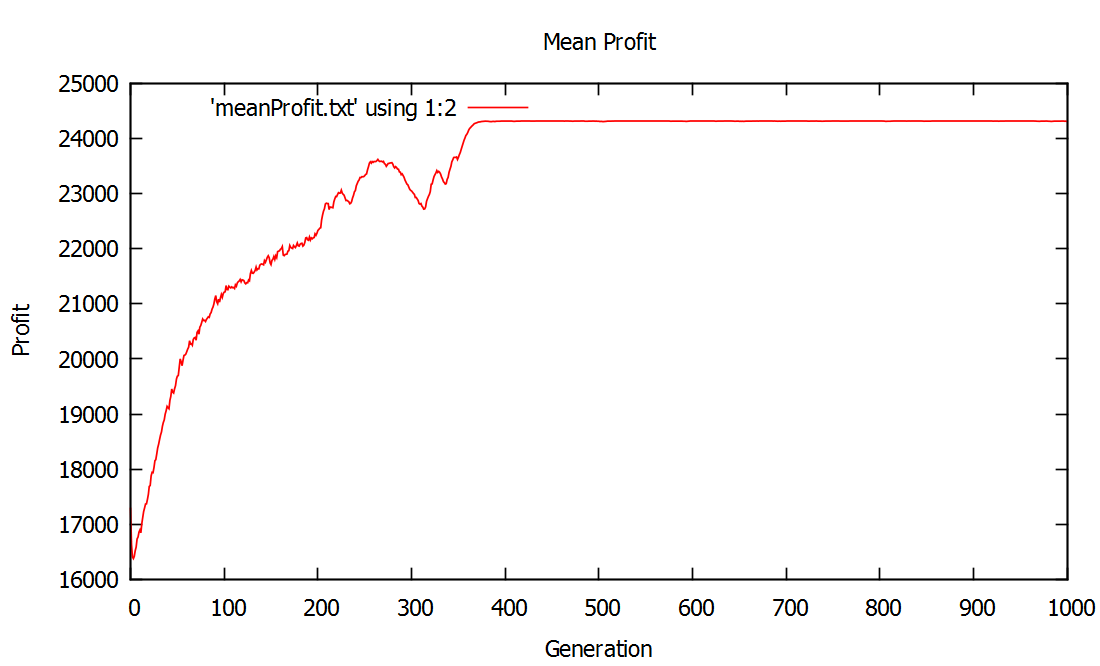
\includegraphics[width=400px]{images/population-high.png}
	\caption{High population size}
	\label{fig:population-high}
\end{figure}
This run performs equally as good as the good solution (see \autoref{fig:good-config}), but it takes way more processing time. Instead of 13719ms of the high quality configuration (see \refnn{subsec:good-config}), this one has taken 154519ms, which is \textbf{11 times more}.\\
An approach with a very low population size (10) is shown in \autoref{fig:population-low}.
\begin{figure}[H]
	\centering
	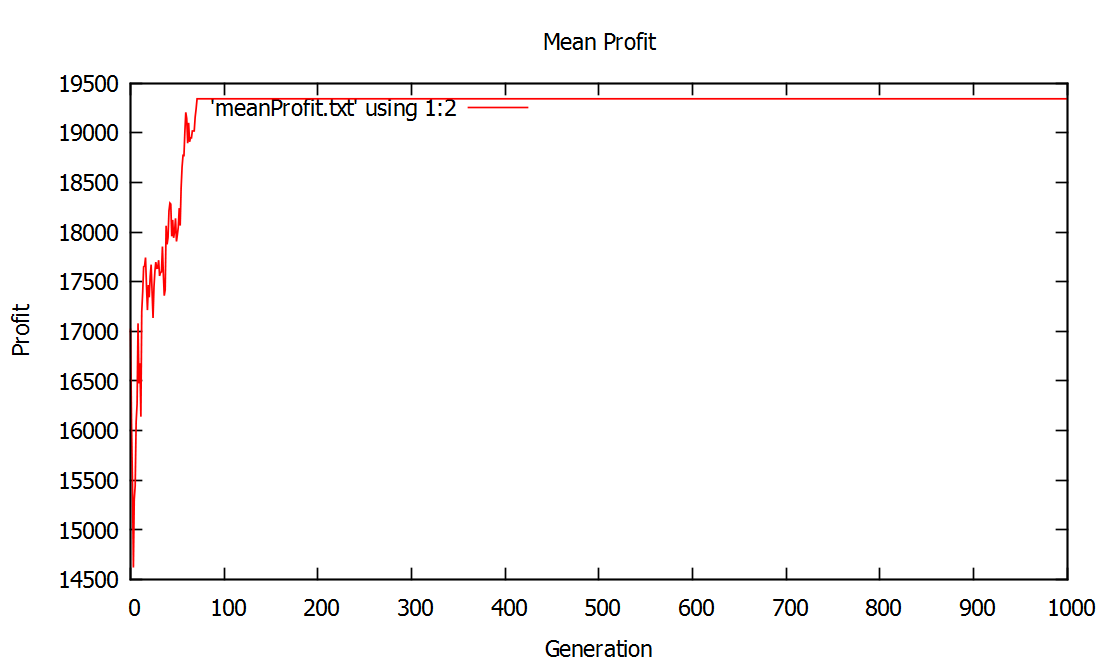
\includegraphics[width=400px]{images/population-low.png}
	\caption{Low population size}
	\label{fig:population-low}
\end{figure}
The graph of \autoref{fig:population-low} converges really fast, due to less individuals to optimize. But the population gets stuck at a local optimum. The graph of \autoref{fig:good-config} converges against about 24000 while \autoref{fig:population-low} converges against about 19400. This approach leads to a suboptimal solution.

\subsection{Generation Count / Duration}
\label{subsec:algorithm-duration}
How high the generation count or duration should be set depends on how much time you are able to wait for the results. More generations lead to a better or optimal solution. Too less generations can lead to a graph that does not reach the optimum. \\
\autoref{fig:generation-low} shows a low generation approach with the following configuration: \\ \\
\begin{tabular}{ |l|l| }
	\hline
	Breed probability & 0.8 \\ \hline
	Mutation probability & 0.0001 \\ \hline
	Generation count & 100 \\ \hline
	Population size & 300 \\ \hline
\end{tabular}
\begin{figure}[H]
	\centering
	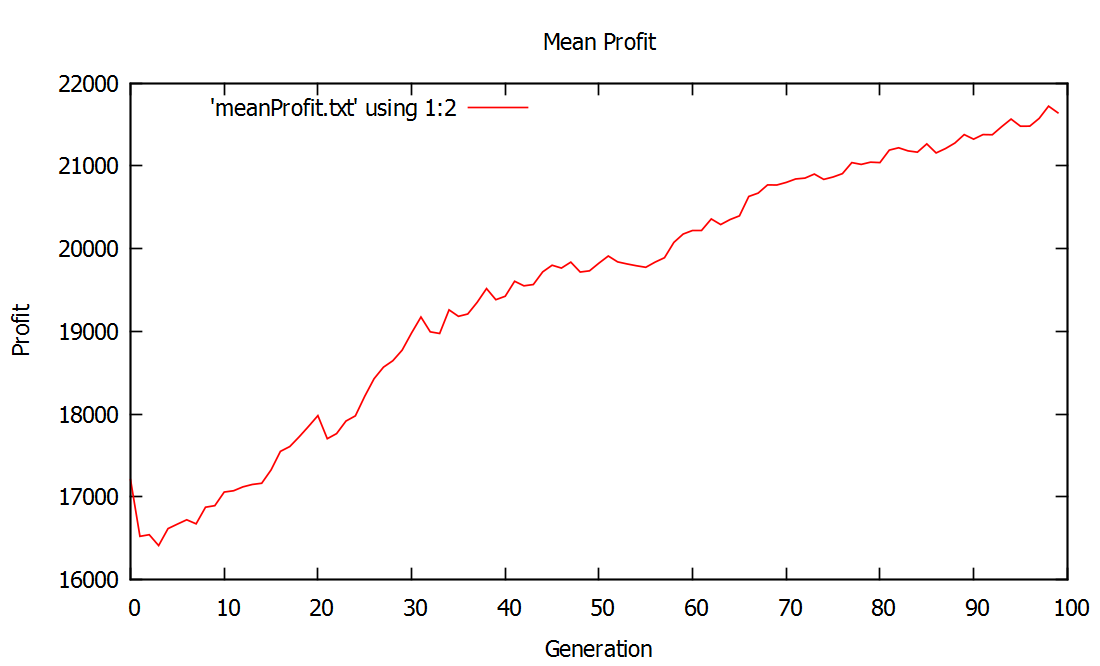
\includegraphics[width=400px]{images/generation-low.png}
	\caption{Low generation count}
	\label{fig:generation-low}
\end{figure}
In comparison to \autoref{fig:good-config} this one does not even nearly reach the optimal value. The graph of \autoref{fig:generation-low} does not converge and shows increasing behaviour. The conclusion is that the solution can be better, if we process more generations.

\chapter{Review}
\label{chap:review}

\section{Implementation}
\label{sec:rev-impl}
Genetic algorithms got really popular these days and there are a lot of papers around, which describe different approaches to solve the knapsackproblem using a genetic algorithm. In the following I will review the paper \textbf{A hybrid genetic algorithm for MKP} \cite{bib:hybrid-ga}. The algorithm described in the mentioned paper also solves a multidimensional knapsack problem with a genetic algorithm but with different implementation of the modules. \\ \\
The fitness function in this approach is realized as the profit of an individual together with a penalty function, if the individual does not meet the constraints \cite[p. 5]{bib:hybrid-ga}. This leads to a population that allows individuals which violate constraints, which is not possible with the "individual repairing" approach (see \refnn{sec:implementation}). \\ \\
Parent individuals are selected using stochastic universal sampling (SUA). The individuals are mapped onto the interval $[0,1]$ with a length corresponding to their fitness value. Then N parents are chosen. The first individual is selected by generating a random number in the interval $[0,1/N]$, then iterative add $1/N$ to the random number until we got N individuals \cite[p. 5 - 6]{bib:hybrid-ga}. This is different in performance compared to the roulette wheel selection, which generates a random number for each individual (see \refnn{sec:implementation}). Generating a random number takes a lot of time, so SUA should be faster than the roulette experiment. \\ \\
Generating the initial population is done with the Dantzig algorithm. This algorithm generates the $profit/weight$ ratio for each item and sorts them descending. In each step the item with the highest ratio is added to the individual, if it does not collide with the constraints, else the next best item is taken. In the multidimensional knapsackproblem the Dantzig algorithm is coupled with each constraint \cite[p. 6 - 7]{bib:hybrid-ga}. This may result in a initial population with much fitter individuals than the pure random approach (see \refnn{sec:implementation}), but the diversity of genes is much lower. \\ \\
In this genetic algorithm implementation M-point-crossover is used to generate children \cite[p. 7]{bib:hybrid-ga}. \\ \\
For the mutation step, initially a rather small mutation probability is chosen, which increases with each iteration. During the mutation step a random number is generated for each gene of the individual. If the number is smaller or equal to the mutation probability, the gene is flipped \cite[p. 7 - 8]{bib:hybrid-ga}. In this case every gene has the chance to mutate. The result is that there can be multiple genes in one mutation step of one individual, that mutate. In my approach only one gene can flip at each mutation step for each individual. This leads to less randomness than in the algorithm of Djannaty and Doostdar, but it can take longer to escape from a local optimum. 

\section{Conclusion}
\label{sec:rev-con}
In my opinion this is a really interesting and quite different genetic algorithm compared to mine. I had a hard time to find an efficient way to repair the individuals. In the end I got stuck with randomly removing genes until the individual meets the constraints. In the reviewed paper no repairing is done at all, instead a penalty function is used to let the algorithm do the repairing over time by itself. \\
Another really intersting approach is parent selection using stochastic universal sampling. This selection method takes much less computation time and still respects the fitness of each individual. \\

\begin{thebibliography}{999}
	\raggedright
	\bibitem{bib:hybrid-ga} A hybrid genetic algorithm for MKP, Farhad Djannaty, Saber Doostdar \url{http://www.m-hikari.com/ijcms-password2008/9-12-2008/djannatyIJCMS9-12-2008.pdf}, 18.06.2014
\end{thebibliography}

\cleardoublepage
\addcontentsline{toc}{chapter}{\listfigurename}
\listoffigures

\end{document}